\chapter{台虎钳零件三维建模}
台虎钳,又称虎钳,是用来夹持工件的通用夹具。一般装置在工作台上,用以夹稳加工工件,为钳工车间必备工具。它的结构是由钳体、底座、导螺母、丝杠、钳口体等组成。活动钳身通过导轨与台虎钳台虎钳固定钳身的导轨作滑动配合。丝杠装在活动钳身上,可以旋转,但不能轴向移动,并与安装在固定钳身内的丝杠螺母配合。当摇动手柄使丝杠旋转,就可以带动活动钳身相对于固定钳身作轴向移动,起夹紧或放松的作用。其结果如图\ref{fig:taihuqianjiegou} 所示。

\begin{figure}[htbp]
\centering
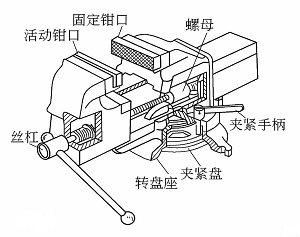
\includegraphics[width=0.8\textwidth]{taihuqianjiegou.png}
\caption{台虎钳结构图}\label{fig:taihuqianjiegou}
\end{figure}

本章选取台虎钳中比较典型的零件进行三维建模,并以此进一步学习与之相关的AutoCAD三维命令和三维建模技巧,学习新的机械图样表达方法和相关规定,了解螺纹的相关知识和图样表达规定。其具体内容有:
\begin{itemize}
\item 台虎钳典型零件的三维建模
\item 半剖视图的制作
\item 阶梯剖视图的制作
\item 剖面视图的制作
\item 螺纹的相关知识
\end{itemize}

%\chapter{圆螺丝钉}

\endinput
%\section{丝杠}

\endinput
%\chapter{滑块}

\endinput
%\chapter{动掌}

\endinput
%\chapter{底座}

\endinput
%\chapter{台虎钳装配}

\endinput

\endinput